\def\passo{1}\def\id#1{#1}%
\newcommand{\cell}[2][\vphantom{$\id{R}$}]{\shortstack{\small #1 \\ \tiny $#2$}}%
\def\chave#1{[#1]}
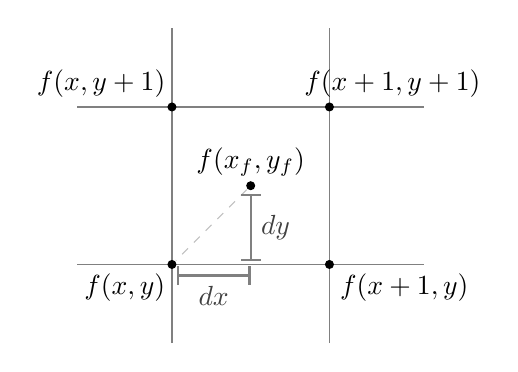
\begin{tikzpicture}
    \draw[step=\passo*2cm,color=gray] (-1.2*\passo,-1*\passo) grid (3.2*\passo,3*\passo);

    \node [fill,draw,circle,inner sep=1pt] at (0*\passo,0*\passo) {};
    \node at (-0.6*\passo,-0.3*\passo) {$f(x, y)$};
    \node [fill,draw,circle,inner sep=1pt] at (2*\passo,0*\passo) {};
    \node at (2.95*\passo,-0.3*\passo) {$f(x+1, y)$};
    \node [fill,draw,circle,inner sep=1pt] at (0*\passo,2*\passo) {};
    \node at (-0.9*\passo,2.3*\passo) {$f(x, y+1)$};
    \node [fill,draw,circle,inner sep=1pt] at (2*\passo,2*\passo) {};
    \node at (2.8*\passo,2.3*\passo) {$f(x+1, y+1)$};

    \node [fill,draw,circle,inner sep=1pt] at (1*\passo,1*\passo) {};
    \node at (1*\passo,1.3*\passo) {$f(x_f, y_f)$};

    \draw [color=lightgray,thin,dashed] (1*\passo - 0.05*\passo, 1 *\passo - 0.05*\passo) -- (0*\passo + 0.05*\passo, 0*\passo + 0.05*\passo);

    \draw [color=gray,thick,|-|] (1*\passo, 1 *\passo - 0.1*\passo) -- (1*\passo, 0*\passo + 0.04*\passo) node[midway, right, color=darkgray] {$dy$};
    \draw [color=gray,thick,|-|] (1*\passo - 0*\passo, -0.14 *\passo) -- (0*\passo + 0.06*\passo, -0.14*\passo) node[midway, below, color=darkgray] {$dx$};
\end{tikzpicture}
